\section{Unbalanced Tree Search (UTS)}
\label{sec:uts}

The UTS benchmark measures the rate of traversal of a
tree generated on the fly using a splittable random number generator
\cite{lcpc06}. The problem specification describes several cryptographic laws
for computing the number of children of a node and their hashes. This results in
trees that are deterministic but unbalanced in unpredictable ways. 

A sequential implementation of UTS is straightforward: the code maintains a
work list of nodes to expand, and repeatedly pops one and adds its children to
the list. It terminates when the list is empty. %, and returns the number of popped elements.
In contrast, a parallel and distributed implementation of UTS
is a challenge because of imbalance. We implement distributed work stealing
with lifelines \cite{ppopp11}.

\paragraph{Distributed Algorithm.} A fixed collection of workers collaborate on
the traversal. The workers are organized in a ring. Each worker maintains a
work list of pending nodes to visit and count of nodes already traversed. Each
worker primarily processes its own list, following the sequential algorithm. If
the list becomes empty, the worker tries to steal nodes from another random
worker. If this fails because the victim's work list is empty as well, the
worker sends a request to the next worker in the ring---its lifeline---and
stops. If this lifeline now has or later obtains nodes to process, it deals a
fraction of these nodes to the requester. One work list is initialized with the
root node of the traversal. The traversal is complete when all workers have
stopped and there are no deal messages from a lifeline in flight. The sum of
the node counts is computed at that point.

Each worker can be in one of three states; \lstinline{work}: the worker is processing nodes from its work list,
\lstinline{wait}: the worker is attempting to steal nodes from a random victim and waiting for the result, and
\lstinline{idle}: the worker has signaled its lifeline and stopped.

% Figure~\ref{fig:uts-state} shows these states and the possible transitions as a
% graph. The transitions---the edges---are annotated with the events associated
% with them. E.g., the \lstinline{NoDeal}/\lstinline{LifelineReq} transition from
% the wait state to the idle state denotes that this transition takes places upon
% receiving the \lstinline{NoDeal} message and involves sending the \lstinline{LifelineReq}
% message.
% \begin{figure}
% \centering
% \begin{tikzpicture}[scale=0.15]
% \tikzstyle{every node}+=[inner sep=0pt]
% \draw [black] (16.5,-13.6) circle (3);
% \draw (16.5,-13.6) node {\lstinline{idle}};
% \draw [black] (35.5,-13.6) circle (3);
% \draw (35.5,-13.6) node {\lstinline{work}};
% \draw [black] (54.6,-13.6) circle (3);
% \draw (54.6,-13.6) node {\lstinline{wait}};
% \draw [black] (19.093,-12.1) arc (114.8182:65.1818:16.454);
% \fill [black] (32.91,-12.1) -- (32.39,-11.31) -- (31.97,-12.22);
% \draw (26,-10.08) node [above] {/\lstinline{LifelineDeal}};
% \draw [black] (38.101,-12.113) arc (114.61614:65.38386:16.684);
% \fill [black] (52,-12.11) -- (51.48,-11.32) -- (51.06,-12.23);
% \draw (45.05,-10.1) node [above] {\lstinline{Steal}/};
% \draw [black] (38.443,-13.022) arc (99.06897:80.93103:41.916);
% \fill [black] (38.44,-13.02) -- (39.31,-13.39) -- (39.15,-12.4);
% \draw (45.05,-13.1) node [below] {/\lstinline{Deal}};
% \draw [black] (51.81,-14.703) arc (-70.22137:-109.77863:48.053);
% \fill [black] (19.29,-14.7) -- (19.87,-15.44) -- (20.21,-14.5);
% \draw (35.55,-18.04) node [below] {\lstinline{LifelineReq}/\lstinline{NoDeal}};
% \draw [black] (9.3,-13.6) -- (13.5,-13.6);
% \fill [black] (13.5,-13.6) -- (12.7,-13.1) -- (12.7,-14.1);
% \end{tikzpicture}
% \caption{State diagram for UTS workers.\label{fig:uts-state}}
% \end{figure}

\paragraph{Implementation in \apgas.} We focus here on two aspects of the
implementation: active messages and termination. Figure~\ref{fig:utsapgas}
shows a fraction of the \lstinline{Worker} class.
%  Each worker holds a boolean
% indicating whether the lifeline has been activated by the previous worker in
% the ring.
When a worker has run out of work and stealing has failed, the protocol
dictates that it goes into \lstinline{idle} mode and signals the next worker in
the ring that it has done so. This corresponds in the code to the completion of
the \lstinline{run()} task by the invocation of \lstinline{lifelineReq()}. This
second method implements an active message pattern: the execution of
\lstinline{lifeline.set(true)} happens at place \lstinline{nextInRing}. This
works because the implicit \lstinline{this} captured in the closure has type
\lstinline{PlaceLocal} and is therefore resolved to the \lstinline{Worker}
instance unique to the destination place.
\begin{figure}
\begin{lstlisting}
class Worker($\ldots$) extends PlaceLocal {
  val workList: WorkList $\EQ$ $\ldots$
  val lifeline: AtomicBoolean $\EQ$ $\ldots$
  $\ldots$
  def run() : Unit $\EQ$ {
    synchronized { state $\EQ$ Work }
    while ($\ldots$) {
      /* Work while work is available and/or stealing
         is successful. */ $\ldots$ }
    synchronized { state $\EQ$ Idle }
    lifelineReq() }
  def lifelineReq() : Unit $\EQ$ {
    asyncAt(nextInRing) { lifeline.set(true) } }
  def lifelineDeal(work: Worklist) : Unit $\EQ$ {
    workList.merge(Worklist)
    run()
} }
\end{lstlisting}
\caption{Selected code structure for UTS in \apgas.\label{fig:utsapgas}}
\end{figure}
Reactivation of a worker that has gone idle is achieved in a similar way; its
lifeline runs:
\begin{lstlisting}
  asyncAt(prevInRing) { lifelineDeal(newWork) }
\end{lstlisting}
This, as shown in Figure~\ref{fig:utsapgas}, spawns a task that enters
\lstinline{run()}.

Distributed termination detection is notoriously difficult to implement
correctly and efficiently. For instance in UTS, observing that all workers are
idle does not guarantee that the traversal is complete as messages containing
nodes to process might still be in flight. In our code, however, a single
invocation of \lstinline{finish} solves the problem.
We invoke our distributed computation from the first place as
\begin{lstlisting}
  finish { worker.run() }
\end{lstlisting}
As shown in Figure~\ref{fig:utsapgas}, when a worker goes into \lstinline{idle}
mode, the corresponding task completes. Since \lstinline{finish} guards all
tasks transitively, it terminates exactly when the last work item has been
exhausted.

% APGAS provides two state-of-the-art \lstinline{finish} implementations for
% fault-tolerant and non-fault-tolerant instantiations of the library. The core
% algorithm uses a distributed array of counters akin to the X10 implementation.
% Each place maintains the count of tasks that completed locally and separate
% counts for each place where it spawned tasks. These arrays of counters are
% pushed to the place of the task waiting on the \lstinline{finish}. Termination
% is signaled when all the sums of the per-place task counts are zero.

\paragraph{Implementation with Akka.} Because Akka embraces explicit messaging
and actors that act as state machines, the code follows the protocol
description very closely. For instance, the code corresponding to a worker
being reactivated by its lifeline is:
\begin{lstlisting}
  case LifelineDeal(wl) $\RA$
    workList.merge(wl); become(working); self ! Work
\end{lstlisting}
A significant challenge, however, lies in detection termination. We implemented
a protocol where workers that go into \lstinline{idle} mode additionally
communicate to a central worker how many times they have sent lifeline
messages, and by aggregating all counts, the central worker can detect when no
messages are in flight.

% TODO
% 
% Common implementation of WorkList. Show interface. Explain mutability and
% ownership are for performance.
% 
% Akka: implementation using vanilla actors (no akka-fsm). Work is split up by
% sending \lstinline{Work} messages to oneself. State transitions are implemented
% using \lstinline{become}.
% 
% Termination is difficult.
% 
% UTS: three problems, three solutions.
% 
% UTS \apgas: concurrency control implemented as multiple paradigms (synchronized
% data access, global invariants, active messages). Concurrency is more
% fine-grained.


% Scala performance

\paragraph{Performance.} We measured the rate of traversal of our Akka and
\apgas implementations of UTS in millions of nodes per second (Mn/s), using
32-way parallelism on a 48 core machine. We measured three configurations: 1)
\apgas implementation on 32 processes, 2) Akka implementation on 1 process with
32 worker actors, 3) Akka implementation on 32 processes, each with 1 worker
actor.\footnote{As places in \apgas are currently only realized as separate
processes, configuration 3) is closer in terms of communication constraints.}
We used \lstinline{akka-remote} for 3), and the flexibility of the actor model
means that the distribution of workers per process is isolated to a single
invocation of \lstinline{.withDeploy}. The configurations achieved 269.4Mn/s,
286.8Mn/s, and 274.2Mn/s, respectively. This shows that the \apgas code comes
within 98\% and 93\% of the performance of the multi-process and single-process
Akka configurations, respectively.

\begin{figure}

\vspace{-0.3cm}
\hspace{-0.4cm}
\begingroup\graphicspath{{figures/}}\section{Unbalanced Tree Search}
\label{sec:uts}

The Unbalanced Tree Search benchmark (UTS) measures the rate of traversal of a
tree generated on the fly using a splittable random number generator
\cite{lcpc06}. The problem specification describes several cryptographic laws
for computing the number of children of a node and their hashes. This results
in trees that are deterministic but unbalanced in unpredictable ways. 

A sequential implementation of UTS is straightforward: the code maintains a
work list of nodes to expand, and repeatedly pops one and adds its children to
the list. It terminates when the list is empty, and returns the number of
popped elements. In contrast, a parallel and distributed implementation of UTS
is a challenge because of imbalance. We implement distributed work stealing
with lifelines \cite{ppopp11}.

\paragraph{Distributed Algorithm.} A fixed collection of workers collaborate on
the traversal. The workers are organized in a ring. Each worker maintains a
work list of pending nodes to visit and count of nodes already traversed. Each
worker primarily processes its own list, following the sequential algorithm. If
the list becomes empty, the worker tries to steal nodes from another random
worker. If this fails because the victim's work list is empty as well, the
worker sends a request to the next worker in the ring---its lifeline---and
stops. If this lifeline now has or later obtains nodes to process, it deals a
fraction of these nodes to the requester. One work list is initialized with the
root node of the traversal. The traversal is complete when all workers have
stopped and there are no deal messages from a lifeline in flight. The sum of
the node counts is computed at that point.

\paragraph{State Machine.} Each worker can be in one of three states:
\begin{itemize}
\item \lstinline{work}: the worker is processing nodes from its work list;
\item \lstinline{wait}: the worker is attempting to steal nodes from a random victim and waiting for the result;
\item \lstinline{idle}: the worker has signaled its lifeline and stopped.
\end{itemize}
Figure~\ref{fig:uts-state} shows these states and the possible transitions as a
graph. The transitions---the edges---are annotated with the events associated
with them. E.g., the \lstinline{NoDeal}/\lstinline{LifelineReq} transition from
the wait state to the idle state denotes that this transition takes places upon
receiving the \lstinline{NoDeal} message and involves sending the \lstinline{LifelineReq}
message.
\begin{figure}
\centering
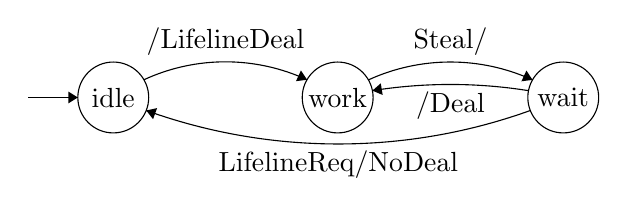
\begin{tikzpicture}[scale=0.15]
\tikzstyle{every node}+=[inner sep=0pt]
\draw [black] (16.5,-13.6) circle (3);
\draw (16.5,-13.6) node {\lstinline{idle}};
\draw [black] (35.5,-13.6) circle (3);
\draw (35.5,-13.6) node {\lstinline{work}};
\draw [black] (54.6,-13.6) circle (3);
\draw (54.6,-13.6) node {\lstinline{wait}};
\draw [black] (19.093,-12.1) arc (114.8182:65.1818:16.454);
\fill [black] (32.91,-12.1) -- (32.39,-11.31) -- (31.97,-12.22);
\draw (26,-10.08) node [above] {/\lstinline{LifelineDeal}};
\draw [black] (38.101,-12.113) arc (114.61614:65.38386:16.684);
\fill [black] (52,-12.11) -- (51.48,-11.32) -- (51.06,-12.23);
\draw (45.05,-10.1) node [above] {\lstinline{Steal}/};
\draw [black] (38.443,-13.022) arc (99.06897:80.93103:41.916);
\fill [black] (38.44,-13.02) -- (39.31,-13.39) -- (39.15,-12.4);
\draw (45.05,-13.1) node [below] {/\lstinline{Deal}};
\draw [black] (51.81,-14.703) arc (-70.22137:-109.77863:48.053);
\fill [black] (19.29,-14.7) -- (19.87,-15.44) -- (20.21,-14.5);
\draw (35.55,-18.04) node [below] {\lstinline{LifelineReq}/\lstinline{NoDeal}};
\draw [black] (9.3,-13.6) -- (13.5,-13.6);
\fill [black] (13.5,-13.6) -- (12.7,-13.1) -- (12.7,-14.1);
\end{tikzpicture}
\caption{State diagram for UTS workers.\label{fig:uts-state}}
\end{figure}
\paragraph{Implementation in \apgas.}

We illustrate below the handling of the \{ \lstinline{Steal}, \lstinline{Deal} \} pair of messages in the \apgas implementation.
\begin{lstlisting}
class Worker($\ldots$) extends PlaceLocal {
  val thieves: ConcurrentLinkedQueue[Place] = $\ldots$
  val workList: WorkList = $\ldots$
  $\ldots$
  def steal() : Unit = {
    val thief: Place = here
    val victim: Place = $\ldots$ // pick randomly
    synchronized { state = Wait(p) }
    uncountedAsyncAt(victim) {
      thieves.add(thief)
    }
    synchronized { while (state.isWait) { wait() } }
  }
  def distribute() : Unit = {
    $\ldots$ 
    while({ p = thieves.poll(); p != null}) {
      val wl = workList.split()

      uncountedAsyncAt(p) {
        synchronized {
          workList.merge(wl)
          state = Work
          notifyAll()
        }
      }
    }
  }
}
\end{lstlisting}

\paragraph{Distributed Termination.} Distributed termination detection is notoriously difficult to implement correctly and efficiently.
For instance in UTS, observing that all workers are idle does not guarantee that the traversal is complete as messages containing nodes to process might still be in flight. Thanks to \lstinline{finish}, an entire class of hard-to-reproduce data races is ruled out by construction in APGAS.
A combination of static and dynamic analyses can bring down the cost of termination detection~\cite{TardieuETAL14X10ApgasAtPetascale}. 

APGAS provides two state-of-the-art \lstinline{finish} implementations for fault-tolerant and non-fault-tolerant instantiations of the library. The core algorithm uses a distributed array of counters akin to the X10 implementation. Each place maintains the count of tasks that completed locally and separate counts for each place where it spawned tasks. These arrays of counters are pushed to the place of the task waiting on the \lstinline{finish}. Termination is signaled when all the sums of the per-place task counts are zero.


% TODO
% 
% Common implementation of WorkList. Show interface. Explain mutability and
% ownership are for performance.
% 
% Akka: implementation using vanilla actors (no akka-fsm). Work is split up by
% sending \lstinline{Work} messages to oneself. State transitions are implemented
% using \lstinline{become}.
% 
% Termination is difficult.
% 
% UTS: three problems, three solutions.
% 
% UTS \apgas: concurrency control implemented as multiple paradigms (synchronized
% data access, global invariants, active messages). Concurrency is more
% fine-grained.


% Scala performance

\paragraph{Performance.} We measured the rate of traversal of our Akka and
\apgas implementations of UTS in millions of nodes per second (Mn/s), using
32-way parallelism on a 48 core machine. We measured three configurations: 1)
\apgas implementation on 32 processes, 2) Akka implementation on 1 process with
32 worker actors, 3) Akka implementation on 32 processes, each with 1 worker
actor.\footnote{As places in \apgas are currently only realized as separate
processes, configuration 3) is closer in terms of communication constraints.}
We used \lstinline{akka-remote} for configuration 3), and the flexibility of
the actor model means that the distribution of workers per process is isolated
to a single invocation of \lstinline{.withDeploy}. The configurations achieved
269.4Mn/s, 286.8Mn/s, and 274.2Mn/s, respectively. This shows that the \apgas
code comes within 98\% and 93\% of the performance of the multi-process and
single-process Akka configurations, respectively.

%UTSAPGAS 32 places, 1 worker/place, depth 15
%[uts-apgas-32] depth: 15, performance: 4230646601/15.617225935 = 270.8961641848719M nodes/s
%[uts-apgas-32] depth: 15, performance: 4230646601/15.757630678 = 268.4824062355144M nodes/s
%[uts-apgas-32] depth: 15, performance: 4230646601/15.730685914 = 268.9422841527087M nodes/s

%UTSAkka 32 process, 1 actor/process, depth 15
%[actors-32] depth: 15, performance: 4230646601/15.605088175 = 271.1068693464784M nodes/s
%[actors-32] depth: 15, performance: 4230646601/15.478703563 = 273.3204744041263M nodes/s
%[actors-32] depth: 15, performance: 4230646601/15.208430648 = 278.1777225355172M nodes/s

%UTSAkka 1 process, 32 actors, depth 15
%[actors-32] depth: 15, performance: 4230646601/14.622429161 = 289.32584007886373M nodes/s
%[actors-32] depth: 15, performance: 4230646601/14.783925108 = 286.16531605065273M nodes/s
%[actors-32] depth: 15, performance: 4230646601/14.852197401 = 284.8498768751316M nodes/s


%UTSSequential depth 13
%[serial] depth: 13, performance: 264459392/27.782491057 = 9.518922959695061M nodes/s
%[serial] depth: 13, performance: 264459392/27.740853577 = 9.533210334207734M nodes/s
%[serial] depth: 13, performance: 264459392/27.538216937 = 9.603359309900553M nodes/s


% Java performance

%GlobalUTS 32 places, 1 worker/place, depth 15 (hacked non resilient)
%Depth: 15, Places: 32, Performance: 4230646601/15.191 = 278.48M nodes/s using 0 transactions
%Depth: 15, Places: 32, Performance: 4230646601/15.267 = 277.09M nodes/s using 0 transactions
%Depth: 15, Places: 32, Performance: 4230646601/15.138 = 279.46M nodes/s using 0 transactions

%MultiUTS 1 place, 32 workers, depth 15 (hacked non resilient)
%Depth: 15, Locations: 32, Performance: 4230646601/14.601 = 289.73M nodes/s using 0 transactions
%Depth: 15, Locations: 32, Performance: 4230646601/14.791 = 286.02M nodes/s using 0 transactions
%Depth: 15, Locations: 32, Performance: 4230646601/14.557 = 290.61M nodes/s using 0 transactions

%GlobalUTS 32 places, 1 worker/place, depth 15 (resilient map)
%Depth: 15, Places: 32, Performance: 4230646601/15.883 = 266.35M nodes/s using 1119 transactions

\endgroup
\vspace{-0.2cm}
\caption{Weak scaling.}
\label{fig:uts-scaling}
\end{figure}

%UTSAPGAS 32 places, 1 worker/place, depth 15
%[uts-apgas-32] depth: 15, performance: 4230646601/15.617225935 = 270.8961641848719M nodes/s
%[uts-apgas-32] depth: 15, performance: 4230646601/15.757630678 = 268.4824062355144M nodes/s
%[uts-apgas-32] depth: 15, performance: 4230646601/15.730685914 = 268.9422841527087M nodes/s

%UTSAkka 32 process, 1 actor/process, depth 15
%[actors-32] depth: 15, performance: 4230646601/15.605088175 = 271.1068693464784M nodes/s
%[actors-32] depth: 15, performance: 4230646601/15.478703563 = 273.3204744041263M nodes/s
%[actors-32] depth: 15, performance: 4230646601/15.208430648 = 278.1777225355172M nodes/s

%UTSAkka 1 process, 32 actors, depth 15
%[actors-32] depth: 15, performance: 4230646601/14.622429161 = 289.32584007886373M nodes/s
%[actors-32] depth: 15, performance: 4230646601/14.783925108 = 286.16531605065273M nodes/s
%[actors-32] depth: 15, performance: 4230646601/14.852197401 = 284.8498768751316M nodes/s


%UTSSequential depth 13
%[serial] depth: 13, performance: 264459392/27.782491057 = 9.518922959695061M nodes/s
%[serial] depth: 13, performance: 264459392/27.740853577 = 9.533210334207734M nodes/s
%[serial] depth: 13, performance: 264459392/27.538216937 = 9.603359309900553M nodes/s


% Java performance

%GlobalUTS 32 places, 1 worker/place, depth 15 (hacked non resilient)
%Depth: 15, Places: 32, Performance: 4230646601/15.191 = 278.48M nodes/s using 0 transactions
%Depth: 15, Places: 32, Performance: 4230646601/15.267 = 277.09M nodes/s using 0 transactions
%Depth: 15, Places: 32, Performance: 4230646601/15.138 = 279.46M nodes/s using 0 transactions

%MultiUTS 1 place, 32 workers, depth 15 (hacked non resilient)
%Depth: 15, Locations: 32, Performance: 4230646601/14.601 = 289.73M nodes/s using 0 transactions
%Depth: 15, Locations: 32, Performance: 4230646601/14.791 = 286.02M nodes/s using 0 transactions
%Depth: 15, Locations: 32, Performance: 4230646601/14.557 = 290.61M nodes/s using 0 transactions

%GlobalUTS 32 places, 1 worker/place, depth 15 (resilient map)
%Depth: 15, Places: 32, Performance: 4230646601/15.883 = 266.35M nodes/s using 1119 transactions

